% !TEX root = ../thesis.tex

\chapter{Hintergrund}
\label{background}

\paragraph{Ausblick:}
Zum besseren Verständnis der weiteren Verlaufs dieser Arbeit, dient dieses Kapitel zur Einführung in die zugrundeliegenden Themen. Dazu wird zunächst die featurebasierte Softwareentwicklung erläutert, ehe dann der Themenbereich des Machine Learnings vorgestellt wird. Dazu werden die Klassifikation und die Fehlervorhersage mittels Machine Learning erläutert. Unterstützt werden die Abschnitte von Grafiken zum besseren Verständnis der Zusammenhänge.
\\
\hrule

\section{Featurebasierte Softwareentwicklung}
\label{feat-develop}

Das zentrale Konzept hinter der featurebasierten Softwareentwicklung stellen sogenannte Soft-ware-Produktlinien dar. Wie bereits in der Einleitung erwähnt wurde, beschreiben Software-Produktlinien eine Menge von ähnlichen Softwareprodukten, welche eine gemeinsame Menge von Features sowie eine gemeinsame Codebasis besitzen und sich durch die Auswahl der verwendeten Features unterscheiden, sodass eine breite Variabilität innerhalb einer Produktlinie erreicht werden kann \cite{Apel2013,Thuem2014}.

Der zentrale Prozess der Generierung einer Software-Produktlinie ist in \autoref{fig:spl} dargestellt. Aufgeteilt wird dieser Prozess in das Domain Engineering und das Application Engineering. Im Rahmen des Domain Engineerings wird ein sogenanntes Variabilitätsmodell (Variability Model) erzeugt, welches durch die Kombination der wählbaren Features beschrieben wird \cite{Apel2013}. Gängige Implementationstechniken für Features reichen von einfachen Lösungen durch Annotationen basierend auf Laufzeitparametern oder Präprozessor-Anweisungen bis hin zu verfeinerten Lösungen basierend auf erweiterten Programmiermethoden, wie zum Beispiel Aspektorientierung. In Teilen dieser Implementierungstechniken wird jedes Feature wird als wiederverwendbares Domain Artifact modelliert und gekapselt, welches im Prozess des Application Engineerings in Form einer Konfiguration zusammen mit weiteren Features, im Hinblick auf die gewünschte Funktionalität der Software, ausgewählt werden kann. Ein Software Generator erzeugt dann die gewünschten Softwareprodukte basierend auf den bereits zuvor genannten Implementationstechniken für Features.

\begin{figure}[]
    \centering
    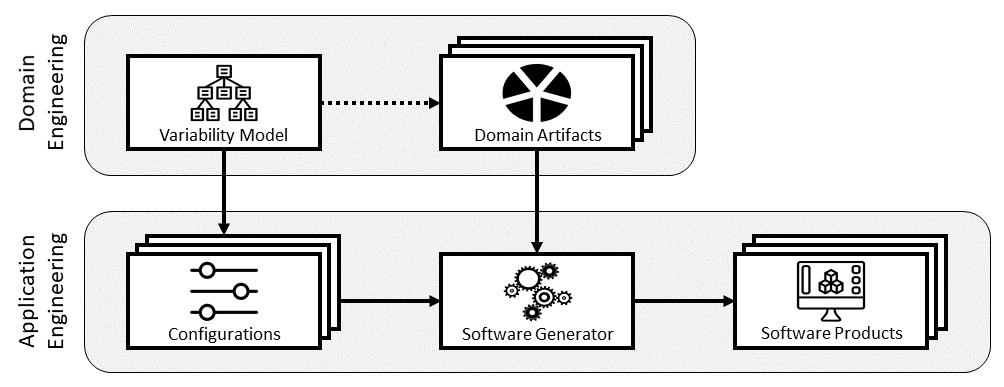
\includegraphics[width=\textwidth]{images/SPL}
    \caption{Generierung von Software-Produktlinien nach \cite{Thuem2014}\label{fig:spl}}
\end{figure}

Die in dieser Arbeit betrachtete Implementierungstechnik von Features basiert auf Anweisungen beziehungsweise Bedingungsdirektiven des C-Präprozessors. Die für diese Arbeit relevanten Direktiven lauten \texttt{\#IFDEF} und \texttt{\#IFNDEF}. Einfache Beispieleinsätze für beide Direktiven sind in \autoref{example1} zu sehen. Sie befinden sich beide innerhalb einer Methode. Die Direktive \texttt{\#IFDEF} leitet den Code der bedingten Gruppe des Features \texttt{feature1} ein, welche mit der Anweisung \texttt{\#ENDIF} endet. Der mit \texttt{//Code feature1} angegebene Codeteil wird genau dann nur ausgeführt, wenn das Feature \texttt{feature1} im Rahmen der Konfiguration des Softwareproduktes definiert beziehungsweise aktiviert ist \cite{Stallmann2016}. In diesem Fall wird die Bedingung der Direktive erfolgreich erfüllt \cite{Stallmann2016}. Sie schlägt fehl, wenn das Feature nicht definiert beziehungsweise aktiviert ist \cite{Stallmann2016}. Die Direktive \texttt{\#IFNDEF} wird für Code verwendet, der ausgeführt werden soll, wenn ein Feature nicht definiert ist. Im Falle des Beispiels wird der in Zeile 7 angedeutete Code nur ausgeführt, wenn \texttt{feature2} nicht aktiviert wurde.
Es besteht zudem die Möglichkeit, Features bzw. ihren Code zu verschachteln. Ein Beispiel dafür ist in \autoref{example2} angegeben. Es ist zu erkennen, dass sich der Code von \texttt{feature2} innerhalb der bedingten Gruppe von \texttt{feature1} befindet. Der in Zeile 5 angedeutete Code kann somit nur ausgeführt werden, wenn \texttt{feature1} aktiviert ist. Im Fall von Verschachtelung beendet ein \texttt{\#ENDIF} immer das nächstgelegene \texttt{\#IFDEF} oder \texttt{\#IFNDEF} \cite{Stallmann2016}. Es besteht zudem die Möglichkeit, Direktiven mittels \glqq und\grqq{} (\texttt{\&\&}, \texttt{and}) oder \glqq oder\grqq{} (\texttt{||}, \texttt{or}) zu erweiterten Bedingungen zu verknüpfen \cite{Stallmann2016}.

\noindent\begin{minipage}{.45\textwidth}
\begin{lstlisting}[caption=Beispieleinsätze von \texttt{\#IFDEF} und \texttt{\#IFNDEF},frame=tlrb,language=C, label=example1]{example1}
void example(){
#IFDEF feature1
	// Code feature1
#ENDIF
// Code
#IFNDEF feature2
	// Code
#ENDIF
// Code
}
\end{lstlisting}
\end{minipage}\hfill
\begin{minipage}{.45\textwidth}
\begin{lstlisting}[caption=Beispiel eines verschachtelten Einsatz von \texttt{\#IFDEF},frame=tlrb,language=C, label=example2]{example2}
void example(){
#IFDEF feature1
	// Code feature1
	#IFDEF feature2
			// Code feature1 & feature2
	#ENDIF // Ende Code feature2
	// Code feature1
#ENDIF // Ende Code feature1
// Code
}
\end{lstlisting}
\end{minipage}

\textbf{HIER!!!}
\cite{Stallmann2016}

\textbf{CROSS-CUTTING FÜHRT ZU WEITCHENDEN FOLGEN -> ILLUSTRATION}

\begin{figure}[H]
    \centering
    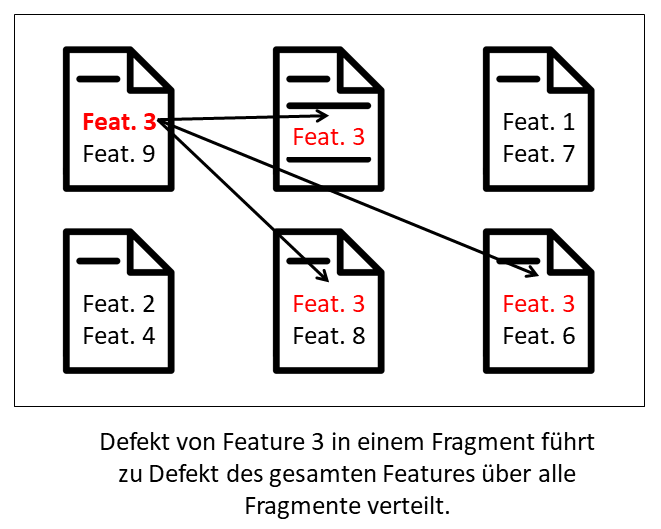
\includegraphics[width=0.6\textwidth]{images/Crosscutting}
    \caption{Auswirkungen eines Defekts in einem Fragment eines Features\label{fig:cross-cutting}}
\end{figure}

\section{Machine-Learning-Klassifikation}
\label{classification}

\textbf{ÜBERARBEITEN!}

Die Machine-Learning-Klassifikation unterliegt dem Teilgebiet des \emph{überwachten Machine Learnings} (englisch: supervised Machine Learning). Die nachfolgende \autoref{fig:ml} präsentiert den allgemeinen Prozess des überwachten Machine Learnings auf vereinfachter Weise anhand eines Beispiels. Anhand dieser werden die wichtigsten Informationen zum genannten Themengebiet erläutert. 

\begin{figure}[H]
    \centering
    \captionsetup{justification=centering,margin=2cm}
    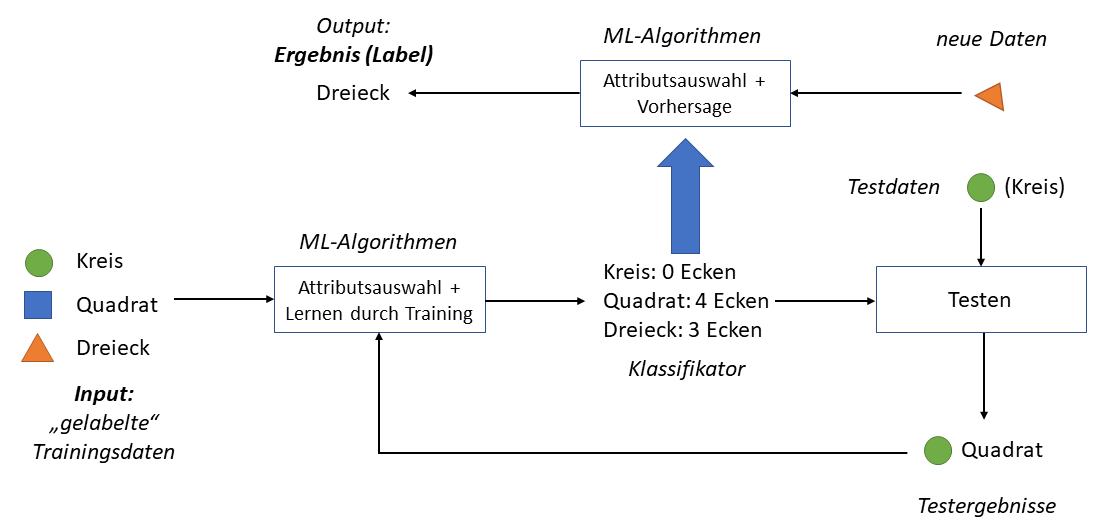
\includegraphics[width=\textwidth]{images/ML}
    \caption{Allgemeiner Prozess des überwachten Machine Learnings dargestellt anhand eines Beispiels (vereinfacht)}\label{fig:ml}
\end{figure}

Das in der Abbildung gezeigte Beispiel zeigt den Prozess der Entwicklung und Erlernung eines Klassifikators zur Erkennung von geometrischen Formen.
Der Prozess beginnt mit der Erstellung eines Datensets, welches als Input für die Erlernung des Klassifikators dient.

\textbf{ÜBERARBEITEN!}

\begin{figure}[H]
    \centering
    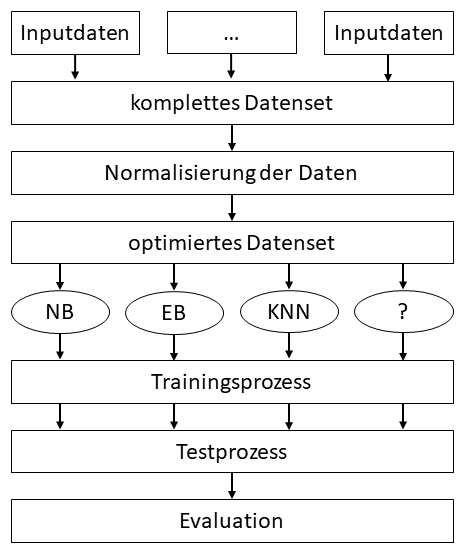
\includegraphics[width=0.5\textwidth]{images/Prozess}
    \caption{Angewendeter Prozess zur Durchführung der Klassfikation nach \cite{Ceylan2006}}\label{fig:process}
\end{figure}

\section{Fehlervorhersage mittels Machine Learning}

Der Hintergrund zur Fehlervorhersage mittels Machine Learning wird anhand eines Beispiels aus der Literatur erläutert. Es stammt aus einer wissenschaftlichen Arbeit von Queiroz et al. \cite{Queiroz2016} und widmet sich der Fehlervorsage von Features. Bei dieser ersten Fallstudie handelt es sich um die bisher einzige Arbeit mit Bezug zu Software-Features und stellt somit für diese Masterarbeit eine bedeutende literarische Grundlage dar. Der Ablauf des von Queiroz et al. angewandten Prozesses zur Erstellung eines featurebasierten Datensets und dessen Anwendung zur Erlernung von Klassifikatoren orientiert sich am zuvor vorgestellten allgemeinen Prozess des überwachten Machine Learnings.

Die Erläuterung des Beispiels erfolgt anhand von drei Abbildungen, welche den in der Arbeit von Queiroz et al. vorgestellten Prozess in drei Teilen visualisieren. 

\begin{figure}[H]
    \centering
    \captionsetup{justification=centering}
    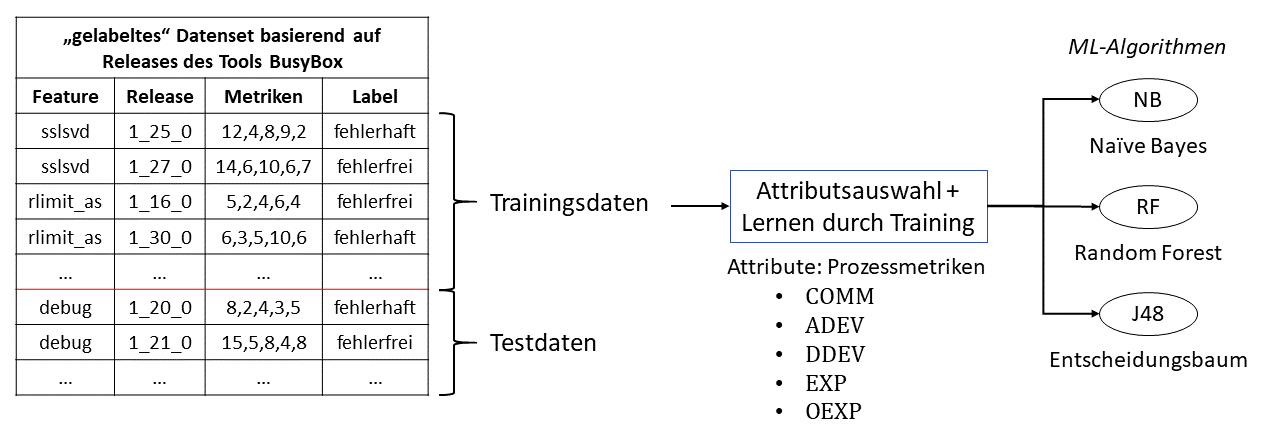
\includegraphics[width=\textwidth]{images/ML1}
    \caption{Teil 1: Featurebasierter Prozess des überwachten Machine Learnings nach \cite{Queiroz2016}}\label{fig:ml1}
\end{figure}

Die Datenbasis des Datensets bilden Commits des UNIX-Toolkits BusyBox\footnote{\url{https://busybox.net/}}, dessen Quellcode frei verfügbar in einem Git-Repository\footnote{\url{https://git.busybox.net/busybox/}} eingesehen und von dort geklont werden kann. Diese Commits wurden wiederum ihren entsprechenden Releases zugeordnet, welche auf der vergebenen Tag-Struktur des Repositories beruhen. Ferner wurden aus den Diffs der Commits die dort bearbeiteten Features extrahiert und anschließend zusammen mit den Release-Informationen in einer MySQL-Datenbank gespeichert. Zusätzlich enthält jeder Datenbankeintrag aggregierte Werte von fünf auf das Feature und den Release bezogenen Prozessmetriken (Erläuterung folgt) sowie das binäre Label, ob ein Feature in einem Release fehlerhaft oder fehlerfrei war. Ein Feature gilt in einem Release als fehlerhaft, sofern in einem Commit des darauffolgenden Releases ein fehlerbehebender Commit bezüglich des Features festgestellt werden konnte. Dies geschieht über die Analyse der Commit-Nachrichten. Sofern eine Commit-Nachricht die Begriffe \glqq bug\grqq{} (Fehler), \glqq error\grqq{} (schwerwiegender Fehler), \glqq fail\grqq{} (fehlschlagen) oder \glqq fix\grqq{} (beheben) enthält, werten die Autoren des Papers den Commit als fehlerbehebend. Alternative Methoden zur Durchführung dieser Analyse bestehen aus der Eindbindung von Daten aus Bug-Tracking-Systemen, die häufig an Software-Repositories angebunden sind, sowie aus der Anwendung des sogenannten SZZ-Algorithmus, welcher in dieser Arbeit verwendet wurde und in \hyperref[szz-def]{Abschnitt 3.2} erläutert wird \cite{Sliwerski2005,Zimmermann2007}. Wie im Rahmen des überwachten Machine Learning üblich, wird das Datenset in Trainings- und Testdaten in einem Verhältnis von 75:25 geteilt. 

Die Trainingsdaten werden dann den Klassifikatoren zur Erlernung zur Verfügung gestellt. Als Attribute dienen fünf Prozessmetriken mit spezifischer Betrachtung von Software-Features. Tabelle XX gibt einen Überblick über die Beschreibungen dieser. Als Klassifikationsalgorithmen wurden Na\"{\i}ve Bayes, Random Forest und J48-Entscheidungsbäume gewählt. Diese Algorithmen wurden unter anderem auch in dieser Arbeit verwendet. Erläuterungen können in \hyperref[algorithms]{Abschnitt 4.1} gefunden werden.

Wie in Abbildung XX dargestellt ist, wird für jeden Klassifikationsalgorithmus ein Klassifikator erstellt, welcher anschließend getestet und evaluiert wird. Dazu werden die jeweiligen Klassifikatoren auf das Testdatenset angewendet, ohne jedoch die Werte der Zielklassen mit anzugeben. Diese werden im Anschluss an den Klassifikationsvorgang mit den vorhergesagten Werten auf Übereinstimmung verglichen. Anhand dieses Vergleiches können die Genauigkeit sowie weitere Metriken zur Bewertung der Leistung der Klassifikatoren gemessen werden. Eine Übersicht von Evaluationsmetriken kann in \hyperref[eval-metrics]{Abschnitt 5.2.1} gefunden werden.

Die so erstellten Klassifikatoren können dann zur Vorhersage von neuen Daten genutzt werden. Dazu müssen die fünf zuvor genannten Prozessmetriken der neuen Daten berechnet werden. 

\begin{table}
\centering
\caption{Übersicht der von \cite{Queiroz2016} verwendeten Prozessmetriken}
\label{tab:metrics}
\begin{tabular}{|c|l|} 
\hline
\textbf{Metrik}  & \textbf{Beschreibung}  \\ 
\hline
COMM & \begin{tabular}[c]{@{}l@{}}Anzahl der Commits, die in einem Release dem betreffenden \\ Feature gewidmet sind. \end{tabular} \\ 
\hline
ADEV & \begin{tabular}[c]{@{}l@{}}Anzahl der Entwickler, die das betreffende Feature\\in einem Release bearbeitet haben. \end{tabular} \\ 
\hline
DDEV & \begin{tabular}[c]{@{}l@{}}kummulierte Anzahl der Entwickler, die das betreffende Feature\\in einem Release bearbeitet haben. \end{tabular} \\ 
\hline
EXP & \begin{tabular}[c]{@{}l@{}}Geometrisches Mittel der „ Erfahrung“ aller Entwickler, die am \\ betreffenden Feature in einem Release gearbeitet haben. \end{tabular} \\ 
\hline
OEXP & \begin{tabular}[c]{@{}l@{}}„ Erfahrung“ des Entwicklers, der am meisten zum betreffenden \\ Feature in einem Release beigetragen hat. \end{tabular} \\ 
\hline
\multicolumn{2}{|c|}{\begin{tabular}[c]{@{}c@{}}Erfahrung ist definiert als Summe der geänderten, gelöschten\\oder hinzugefügten Zeilen im zugehörigen Release. \end{tabular}} \\
\hline
\end{tabular}
\end{table}

\begin{figure}[H]
    \centering
    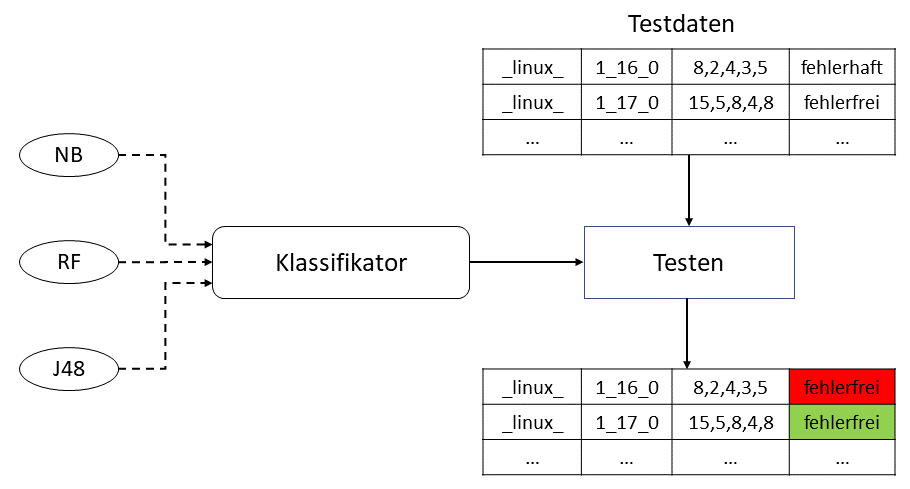
\includegraphics[width=\textwidth]{images/ML2}
    \caption{Teil 2: Featurebasierter Prozess des überwachten Machine Learnings nach \cite{Queiroz2016}}\label{fig:ml2}
\end{figure}

\cleardoublepage
